%!TEX root = ../report.tex

\chapter{Evaluation}
\label{chap:evaluation}

\section{Implementation and measurements.}

\begin{itemize}
 \item Compare based on AUC
 \item What is roc AUC
 \item AUC vs Accuracy, why AUC is better than Accuracy or other point based methods.
 %\item Implementation details of all three structures here with explanation
 %\item Implementation from where why chose this one
 %\item modifications made and why
 \item Talk about tensors, tensorflow and keras here too
 \item Criteria of comparison, mainly the mean AUC then max AUC, then number of parameters and execution time*
\end{itemize}

%\section{Contrastive loss}

\subsection{Search for best hyperparameters}
What are the hyperparameters.
Effect of setting best hyper parameters.

\begin{figure}[ht]
\centering
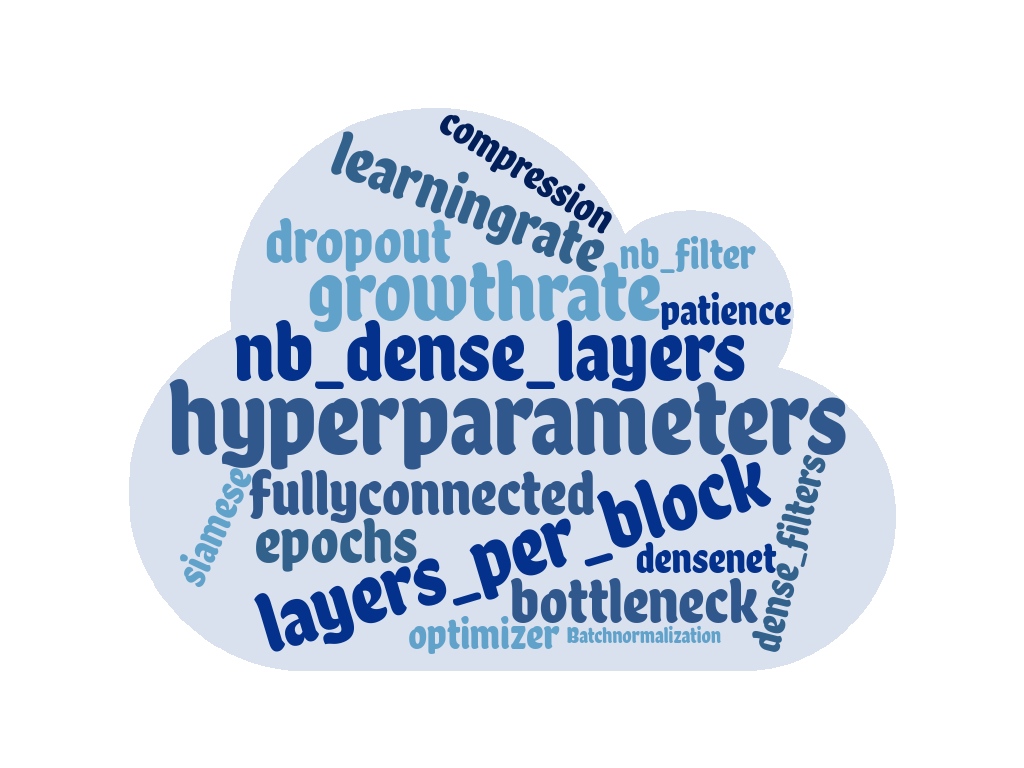
\includegraphics[width=0.5\textwidth]{images/densenet/wordcloud_hyperparameters.png}
\caption{\label{fig:wordcloud_hp}Hyper parameters word cloud.}
\end{figure}

\subsection{Grid search}
Currently the search space for the evaluation is hand designed and supplied to the evaluation script externally. Example
%\begin{figure}[ht]
%\centering
%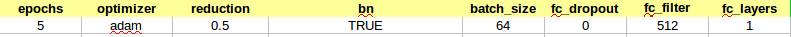
\includegraphics[width=1\textwidth]{images/densenet/test_cases.png}
%\caption{\label{fig:search_space}Custom grid search space example.}
%\end{figure}

\begin{table}
\centering
    \begin{tabular}{|c c c c c|} 
      \hline\hline
      Epochs & Optimizer & Batch size & Dropout & Use batch norm\\[0.5ex] 
      \hline
      5 & adam & 64 & 0.4 & True \\  
      \hline
      5 & adam & 64 & 0.4 & False \\ 
      %\hline
      %5 & adam & 64 & 0.7 & False \\ 
      %\hline
      %8 & rmsprop & 64 & 0.4 & True\\ 
      \hline \hline
    \end{tabular}
  \caption{Custom grid search space example.}
  \label{table:grid_example}
\end{table}

In this example it is displayed that how the search space is hand designed to evaluate different cases, here the effect of using batch normalization can be investigated by comparing the results of two test cases.
All the values set in the grid passed as input to the actual code and defines the structure or different parameters from inside  the code. In \ref{table:grid_example} the flag use batch norm is set to 'True', which
gets propagated in the actual block of code where it enables the use of batch normalization layer, where applicable. 

For the evaluation the epochs are set after multiple testings in order to ensure, to some extend, the networks does not get too overtrained and the generalization gets poorer. Also if the network is undertrained, then 
it will not generalize well. The setting the epochs were one of the big challenge of this work, because in some cases the networks gets overtrained after 4-5 epochs.

\subsection{Training process}
The train data has been divided into train and validation data randomly using sklearn train test data split \cite{sklearnsplit} in 8:2 ratio. This is done using fixed seed to ensure the validation and train cases are 
same for all the evaluations across all three methods. It is important to clarify that the roles of the validation data in keras 
is different than classic training method. In keras the validation data is not used to update the weights. Instead this validation dataset can be used to monitor the network performance in terms of 
validation accuracy and validation loss. Using callback functions such as \code{EarlyStopping} and \code{ReduceLROnPlateu} \cite{kerascallbacks} the network validation performance can be monitored after each epochs of training.
By configuring the callbacks properly (parameter: Early stop patience) the training can be stopped if the validation accuracy or loss does not improve after a number of epochs then the training process terminates.
Similarly, if the validation performance does not improve after some epochs the learning rate can be reduced by a previously determined factor using \code{ReduceLROnPlateu} to come out of the local minima. The patience values 
are set after some manual trials. \\

\begin{lstlisting}
#Early stopping
es = EarlyStopping(monitor='val_acc', patience=es_patience,verbose=1)
#Model check point
checkpointer = ModelCheckpoint(filepath=weight_file, verbose=2, save_best_only=True) 
#Learning rate reducer on plateu
lr_reducer = ReduceLROnPlateau(monitor='val_loss', factor=np.sqrt(0.1), cooldown=0, patience=lr_patience, min_lr=0.5e-6,verbose=1)
\end{lstlisting}

%\code{es = EarlyStopping(monitor='val\_acc', patience=es\_patience,verbose=1)} \\
%\code{checkpointer = ModelCheckpoint(filepath=weight\_file, verbose=2, save\_best\_only=True)} \\
%\code{lr\_reducer = ReduceLROnPlateau(monitor='val\_loss', factor=np.sqrt(0.1), cooldown=0, patience=lr\_patience, min\_lr=0.5e-6,verbose=1)}\\

